\documentclass[runningheads,a4paper]{llncs}\usepackage[]{graphicx}\usepackage[]{color}
%% maxwidth is the original width if it is less than linewidth
%% otherwise use linewidth (to make sure the graphics do not exceed the margin)
\makeatletter
\def\maxwidth{ %
  \ifdim\Gin@nat@width>\linewidth
    \linewidth
  \else
    \Gin@nat@width
  \fi
}
\makeatother

\definecolor{fgcolor}{rgb}{0.345, 0.345, 0.345}
\newcommand{\hlnum}[1]{\textcolor[rgb]{0.686,0.059,0.569}{#1}}%
\newcommand{\hlstr}[1]{\textcolor[rgb]{0.192,0.494,0.8}{#1}}%
\newcommand{\hlcom}[1]{\textcolor[rgb]{0.678,0.584,0.686}{\textit{#1}}}%
\newcommand{\hlopt}[1]{\textcolor[rgb]{0,0,0}{#1}}%
\newcommand{\hlstd}[1]{\textcolor[rgb]{0.345,0.345,0.345}{#1}}%
\newcommand{\hlkwa}[1]{\textcolor[rgb]{0.161,0.373,0.58}{\textbf{#1}}}%
\newcommand{\hlkwb}[1]{\textcolor[rgb]{0.69,0.353,0.396}{#1}}%
\newcommand{\hlkwc}[1]{\textcolor[rgb]{0.333,0.667,0.333}{#1}}%
\newcommand{\hlkwd}[1]{\textcolor[rgb]{0.737,0.353,0.396}{\textbf{#1}}}%

\usepackage{framed}
\makeatletter
\newenvironment{kframe}{%
 \def\at@end@of@kframe{}%
 \ifinner\ifhmode%
  \def\at@end@of@kframe{\end{minipage}}%
  \begin{minipage}{\columnwidth}%
 \fi\fi%
 \def\FrameCommand##1{\hskip\@totalleftmargin \hskip-\fboxsep
 \colorbox{shadecolor}{##1}\hskip-\fboxsep
     % There is no \\@totalrightmargin, so:
     \hskip-\linewidth \hskip-\@totalleftmargin \hskip\columnwidth}%
 \MakeFramed {\advance\hsize-\width
   \@totalleftmargin\z@ \linewidth\hsize
   \@setminipage}}%
 {\par\unskip\endMakeFramed%
 \at@end@of@kframe}
\makeatother

\definecolor{shadecolor}{rgb}{.97, .97, .97}
\definecolor{messagecolor}{rgb}{0, 0, 0}
\definecolor{warningcolor}{rgb}{1, 0, 1}
\definecolor{errorcolor}{rgb}{1, 0, 0}
\newenvironment{knitrout}{}{} % an empty environment to be redefined in TeX

\usepackage{alltt}

\usepackage[latin1]{inputenc}
\usepackage{amssymb}
\usepackage{amsmath}
\setcounter{tocdepth}{3}
\usepackage{graphicx}
\usepackage{multirow}
\usepackage{rotating}
\usepackage{subfigure}
\usepackage{url}
\usepackage{caption}

\newcommand{\keywords}[1]{\par\addvspace\baselineskip
\noindent\keywordname\enspace\ignorespaces#1}

\providecommand{\tabularnewline}{\\}

\graphicspath{{../img/}}
\DeclareGraphicsExtensions{.pdf}
\IfFileExists{upquote.sty}{\usepackage{upquote}}{}
\begin{document}
%\SweaveOpts{concordance=TRUE}



\title{A performance assessment of evolutionary algorithms in
  volunteer computing environments: the importance of entropy} 


% \author{Juan-J.~Merelo \and Paloma de las Cuevas \and Pablo
%   Garc\'ia-S\'anchez \inst{1} \and Mario Garc\'ia-Valdez \inst{2}}

% \institute{Dept. of Computer Architecture and Technology, University
% of Granada, Spain \and
% Dept. of Graduate Studies at Instituto Tecnol\'ogico de Tijuana}

\author{A.U. Thor \and A. N. Otherauthor \and Just A. Nother \inst{1}
  \and Jet A. Nother \inst{2}}

\institute{Invisible University, Frantzia \and
Institute of Higher Studies, Zootropa}


\maketitle

%\thispagestyle{empty}
%\pagestyle{empty}

\begin{abstract}
In a volunteer distributed computing system, users run a program on
their own machine to contribute to a common effort. If the program is
embedded in a web page, collaboration is straightforward, but also ephemeral. In
this paper, we analyze a volunteer evolutionary computing system called
NodIO, by running several experiments, some of them massive. Our
objective is to discover rules that encourage volunteer
participation and also the interplay of these contributions with the
dynamics of the algorithm itself, making it more or less efficient. 
We will show different measures of
participation and contribution to the algorithm and how different 
volunteer usage patterns and tweaks in the algorithm, such as
restarting clients when a solution has been found, contribute to 
improvements and leveraging of these contributions. We will also try
to find out what is the key factor in the early termination of the
experiments, measuring entropy in the contributions and other large
scale indicators. 
\end{abstract}

\section{Introduction}
\label{introduction}

The World Wide Web provides not only a platform for content
distribution, but also, thanks to the maturity and reliability of the
HTTP protocol, an increasingly reliable and high-performance
operating system for running distributed applications. Besides the
protocol itself, there are two factors that contribute to this fact:
the JavaScript virtual machine every browser runs \cite{paulson2005building}
and the simplified standard interface for interacting with servers
exemplified by the REST application interface convention \cite{masse2011rest}.
Thus creating a distributed computing experiment is just a matter of
making a JavaScript application interchange information with a server,
by using REST. From the point of view of the programmer, this involves
relatively common skills and no special libraries, since the
interface is built in the browser, and a simple application that
responds to those requests on the server side; both involve just a few
dozens lines of code additionally to whatever business logic the
application has. But, more importantly and from the point of view of
the user, that application can be run by simply visiting a web page.

Using this approach for creating distributed experiments is called {\em
  volunteer}, {\em cycle-scavenging} or {\em opportunistic} computing
\cite{sarmenta2001volunteer} and it dates back, in different shapes
and underlying mechanisms, to the origin of the web \cite{david-seti:home}. Our interest
here, however, is to use it as a resource for evolutionary
computation, as our group has done for a long time \cite{jj-ppsn98}.

In this line of research that uses volunteer computing for
evolutionary algorithms, there are several pending issues. The first
and maybe most important is approaching volunteer computing as a
socio-technical system \cite{vespignani2009predicting} which integrates
user decisions and behavioral patterns in the system model; this
includes trying to optimize the number of users in a particular
experiment. The second line of research, although related to the
first, is more focused on the evolutionary algorithm itself and how
different design decisions will affect its performance.
% Is it ok that we say that the first line of research is the most important... but then we focus on the second?
We have approached the first issue in our previous work \cite{jj-ppsn98anonymous},
% I have justified to focus, in this case, on the second
but in this paper our focus will be in the second aspect: we will try to
design a decentralized system that, at the same time, is able to use
all available resources for finding the solution of an evolutionary algorithm. This design will be done incrementally by
changing client and the server and measuring its
impact on the overall performance: time and evaluations needed to find
the solution. Eventually, we want to find a system that, whatever the
number of users available to perform the experiment, is able to
maximize their contribution to the evolutionary algorithm, at the same
time that the evolutionary algorithm itself makes the most of those
contributions and is able to find
the solution to the problem in a minimum time and with the least
number of contributions.

The rest of the paper is organized as follows: Next we will briefly
present the state of the art in opportunistic distributed evolutionary
computation (EC). Section \ref{sec:description} will describe the
framework and problem used in the experiments, which are publicly
available under a free license. We will present the results of the
different steps in the incremental design in Section
\ref{sec:experiments}, to finally wrap up with the conclusions. 

%---------------------------------------------------------------
\section{State of the art}
\label{sec:soa}

Volunteer computing involves users deciding to run a program that acts
as a client or as a peer in an experiment
and, as such, has been deployed in many different ways from the
beginning of the Internet, starting with the SETI@home framework for
processing extraterrestrial signals \cite{david-seti:home} or
high-throughput queuing system that such as HTCondor \cite{HTCondor}.
However
the dual facts of the introduction of JavaScript as a universal language for the
browser and the browser itself as an ubiquitous web and Internet client has
made this combination the most popular for volunteer computing
frameworks such as the one we are using here, and whose first version
was described in [citation hidden]. Systems based on the
JavaScript/browser combination
emphasize the ephemerality, ease of use and universality, while
systems such as HTCondor or BOINC might be more adequate for work that
require higher availability of volunteer resources, achieving this
with downloadable clients, in some cases like HTCondor needing
administration access to the resources.
%\cite{DBLP:conf/gecco/GuervosG15}.

Several authors have already described systems using JavaScript  either
for unwitting
\cite{unwitting-ec,boldrin2007distributed} or volunteer 
\cite{langdon:2005:metas,gecco07:workshop:dcor} distributed
evolutionary computation and it has been used ever since by several
authors, including more recent efforts
\cite{duda2013distributed,DBLP:journals/corr/abs-0801-1210,EvoStar2014:jsEO}.

Using a peer to peer approach, the SPACE framework \cite{leclerc2016seamless} distributes fitness 
evaluations across a heterogeneous pool of cloud compute nodes and volunteer
peer computers running a browser. In SPACE peers stablis a bi-directional 
communication with the server using the Socket.io JavaScript library.  
As an experiment they provide an ASM.js compiled version of the RoboGen 
software platform, showing that JavaScript can be used in a broad 
spectrum of applications.  

Recent works have been using crowdsourcing in order to train robots 
for human interaction, a representative work of this trend is that of  
Anetsberger \& Bongard \cite{anetsbergerrobots} in which they propose 
training simulated robots  the grounding of language symbols. They do this by using human 
observers that issue arbitrary commands to these robots via the web, 
providing positive or negative reinforcement in response to the
robot\'s resulting actions. For interaction, they use the Twitch 
video streaming platform where users can issue commands through the
platform's integrated chat service. Subjects were incentivized to 
interact with the system by GUI features that provided participants
with a sense of involvement with the simulation. This kind of systems
could add additional dynamics, because users can collaborate or 
even compete with each other when issuing their commands.


Most
of these papers focused on testing the system by itself as proofs of
concepts, more than on its performance or their actual influence on
the result of an evolutionary algorithm. In fact, some of them do not
even work in as a distributed computing system
\cite{EvoStar2014:jsEO}, describing the expressive capabilities of
JavaScript for evolutionary computation. 


The proof of concepts described above do not go further than trying to
find out  how many users join the effort and how many the system is
able to support. In fact, systems described in
\cite{gecco07:workshop:dcor} had serious scaling issues; some of them
also tried to find out how much time was needed to find the solution
or, alternatively, how many users would be needed to be competitive
with single-user single-computer implementations of the same
algorithm. However, the latest systems try to enphasize the seamless
integration of peer and volunteer computing systems \cite{leclerc2016seamless}. 

This latest system offloads evaluation to browsers so the actual
algorithm runs in some other place; in general, most researchers do
not try to assess the performance of the algorithm 
itself in the precise conditions they find in a volunteer computing
system, although papers such as the one by Laredo et
al. \cite{churn08:ijhpsa}, using models, try to find out the resulting
performance when the users are changing continuously according to a
Weibull distribution. In the case of Klein and Spector \cite{unwitting-ec}, the algorithm
is actually run on the server, using the browser mainly for fitness
evaluation so no actual contribution to the evaluation of the
evolutionary algorithm itself is made.

There is another factor that should be taken into account: since the
user has control of the browser, there is a limited amount of
interaction with it, namely, the fact that by reloading the webpage they
can apply a kind of hypermutation, killing the current population and
generating new individuals some of which will make their way to the
common pool via migration. In that sense, volunteer computing is also
a way of {\em human computation} \cite{quinn2011human}, a concept that
has also been applied to evolutionary algorithms \cite{972056}, in
this case extensively and with all operators. It is quite difficult to
find out how many times this happens and what is their effect on the
overall algorithm, but this only reaffirms the fact that there is a
long list of issues with volunteer evolutionary computation, and that
the volunteer him or herself is at the center of many of them.

In this paper we will make contributions towards the design of
efficient volunteer evolutionary algorithms by studying the effect of
several design decisions on performance. In the next Section we will
present the general framework and the initial setup.


\section{Description of the framework}
\label{sec:description}

In this section we present {\sf NodIO}, a distributed volunteer-based 
evolutionary computation system immplemented in JavaScript. 
All parts of the framework are free and available
with a free license from \url{https://ANONYMOUS-URL}.
%\url{https://github.com/JJ/splash-volunteer}. 

The architecture of the {\sf NodIO} system is divided in two tiers:\begin{enumerate}
\item A REST (representational state transfer) server that responds to
  HTTP requests made by the browsers. These HTTP requests use JSON for information 
  encoding, in this case chromosomes and related
  information sent by the clients and responses returned by the
  server.  The server has the capability to
  run a single experiment, storing the incoming chromosomes in a
  key-value cache that uses as key the chromosome string itself and is
  reset when the solution is found. This cache has a finite 
  size that erases the oldest chromosomes once it has been filled to % Also "it has been filled to its"
  its maximum capacity.  
\item A client that includes the evolutionary algorithm as
  JavaScript code embedded in a web page that displays the fitness and
  other graphs, some
  additional links, and information on the experiment. 
  This code runs
  an evolutionary algorithm {\em island} that starts with a random
  population, then after every 100 generations, it sends the best individual
  back to the server (via a {\tt PUT} request), and then requests a random
  individual back from the server (via a {\tt GET} request). We have
  kept the number of generations between migrations fixed since it is
  a way of finding out how much real work every client is doing. In
  the version of the server used in this paper, we implemented a
  policy by which the combination IP-fitness chromosome could only be
  inserted once into the cache. That means that if a particular IP
  sends the fitness 99 into the server, it will be accepted only
  once. The main intention of this policy was to avoid {\em
    overlapping} of contributions, with clients still running an {\em
    old} run of the experiment contributing after a new one had
  started. This did not completely avoid these contributions: if the
  clients of the {\em old} run increased their new fitness, it would
  still be allowed. 
\end{enumerate}

Figure \ref{fig:system} describes the general system architecture and
algorithm behavior. Different JavaScript libraries, such as JQuery or {\tt
  Chart.js} have been used to build the user interface elements of the
framework, which should be running in \url{http://ANONYMOUS-URL}, 
%\url{http://nodio-jmerelo.rhcloud.com}, 
a free resource hosted in the
OpenShift Platform as a Service\footnote{It is not guaranteed to be running,
or running the same version, when you read this, however; you can always get
the sources from GitHub and set it up yourself.}.
%
\begin{figure}[!t]
\centering
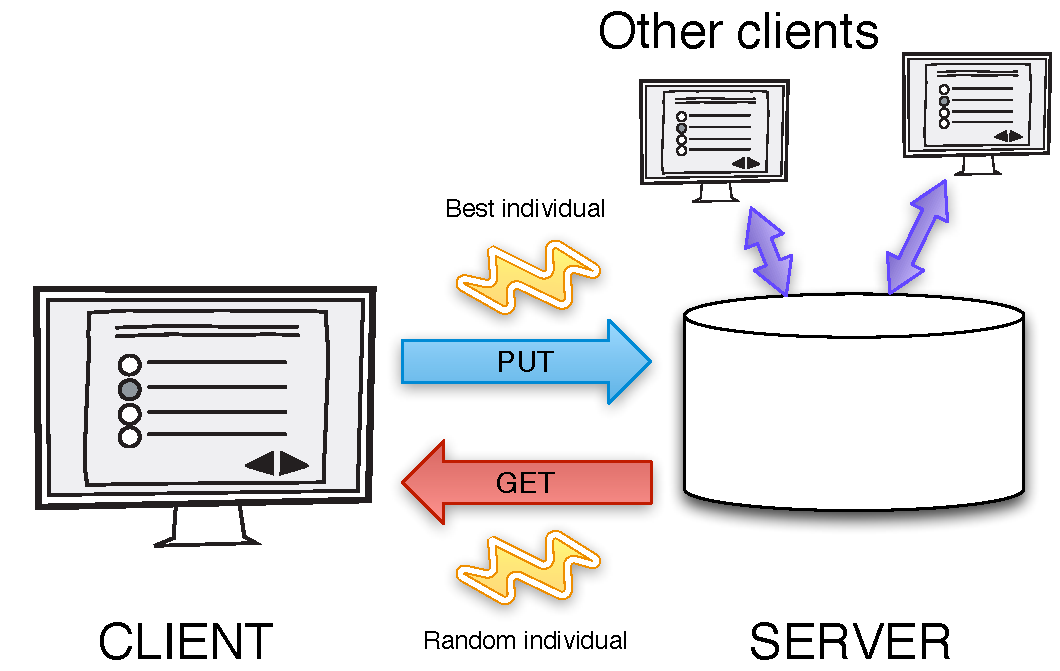
\includegraphics[width=3in]{system.pdf}
\caption{Description of the NodIO system. Clients execute a JavaScript EA
  in the browser, which, every 100 generations, sends the best
  individual and receives a random one back from the server.}
\label{fig:system}
\end{figure}

NodIO needs a fitness function to work with; in this case the classical Trap 
function \cite{Ackley1987} has been used. 
The evolutionary algorithm that uses Trap as fitness function is
completely run in the
browser, but the server needs to know when the solution has been
found, so a subroutine that checks if the solution been found  
is also included in the server, as a configuration
option. In all cases we are using 50 Traps, a problem
that is difficult enough to need the intervention of several users for
an extended amount of minutes.
For every new individual sent by the clients to the cache, several
pieces of metadata are stored: a time stamp, the client IP, the chromosome and
fitness value, the cache size in that particular moment, and also if that
individual actually updated the cache or not. 

All experiments are announced in the same way: we use social networks,
mainly Twitter, to announce the start of a new experiment. LinkedIn,
Facebook, and also private groups in Telegram and WhatsApp have been
used for announcements too. We also encourage friends and followers to
put an original post for announcing it, instead of just sharing, in
the way allowed by the platform, the original post. During the running
of the experiments, users are engaged, questions answered, and all
kind of explanations given if requested. In general, announcements
have been made in Spanish, but in some cases English was used
too. This makes for a certainly unreliable experimentation framework,
but it is a realistic one. The steps in the design of the evolutionary
algorithm will be explained next.

%---------------------------------------------------------------
\section{Experiments and results} 
\label{sec:experiments}

\begin{table}[htb]
\caption{Summary of results for the 5 sets of experiments.\label{tab:runs}}
\begin{center}
\begin{tabular}{|l|c|c|c|c|c|c|c|c|c|}
\hline
Experiment & Median Time & \multicolumn{2}{|c|}{Median IPs} &
\multicolumn{3}{|c|}{Median PUTs} & \#Runs & Unique IPs & Puts/IP \\
           &   (ms)        & Total & Used & Total & Used & Ratio &  & & \\
\hline
base & 120056.0 & 10 & 4 & 256.0 & 21.0 & 0.1290323 & 81 & 262 & 21.33333\\
\hline
graph1 & 152619.5 & 9 & 4 & 212.5 & 26.5 & 0.1282238 & 36 & 96 & 24.30000\\

graph2 & 1173561.5 & 6 & 4 & 761.5 & 22.0 & 0.0520509 & 36 & 73 & 129.04545\\
\hline
reboot & 796214.0 & 9 & 6 & 646.0 & 67.0 & 0.0955121 & 45 & 168 & 75.88889\\
\hline
cachereboot & 392917.0 & 12 & 12 & 576.0 & 79.0 & 0.1575092 & 55 & 225 & 43.28571\\
\hline
\end{tabular}
%% \end{tabular}
%% Initially generated with this code, 
% <<experiments, cache=FALSE,echo=FALSE>>=
%experiment.aggregates$Experiment <- c("base","graph1","graph2","reboot","cachereboot")
%kable(experiment.aggregates)
%@ %def 
\end{center}
\end{table}
%
%
%
Since the point of using a volunteer computing system is to cut costs,
all experiments were set up using the OpenShift
PaaS, which provides a free tier, making the whole experiment cost
equal to nil. In fact, the NodIO system can be deployed to any
Platform or Infraestructure as a Service 
system as long as it can run node.js and can store logs on the same
place or in some other Log as a Service. Local storage can be used,
but it is not a requisite and, in fact, Heroku does not allow
persistent storage of files in its service. 
All these logs are available upon
request. Processed files are available in the same repository that
hosts this paper, as well as the scripts needed to process them. 

%
%
\begin{figure}[htbp]
\centering
\begin{knitrout}
\definecolor{shadecolor}{rgb}{0.969, 0.969, 0.969}\color{fgcolor}
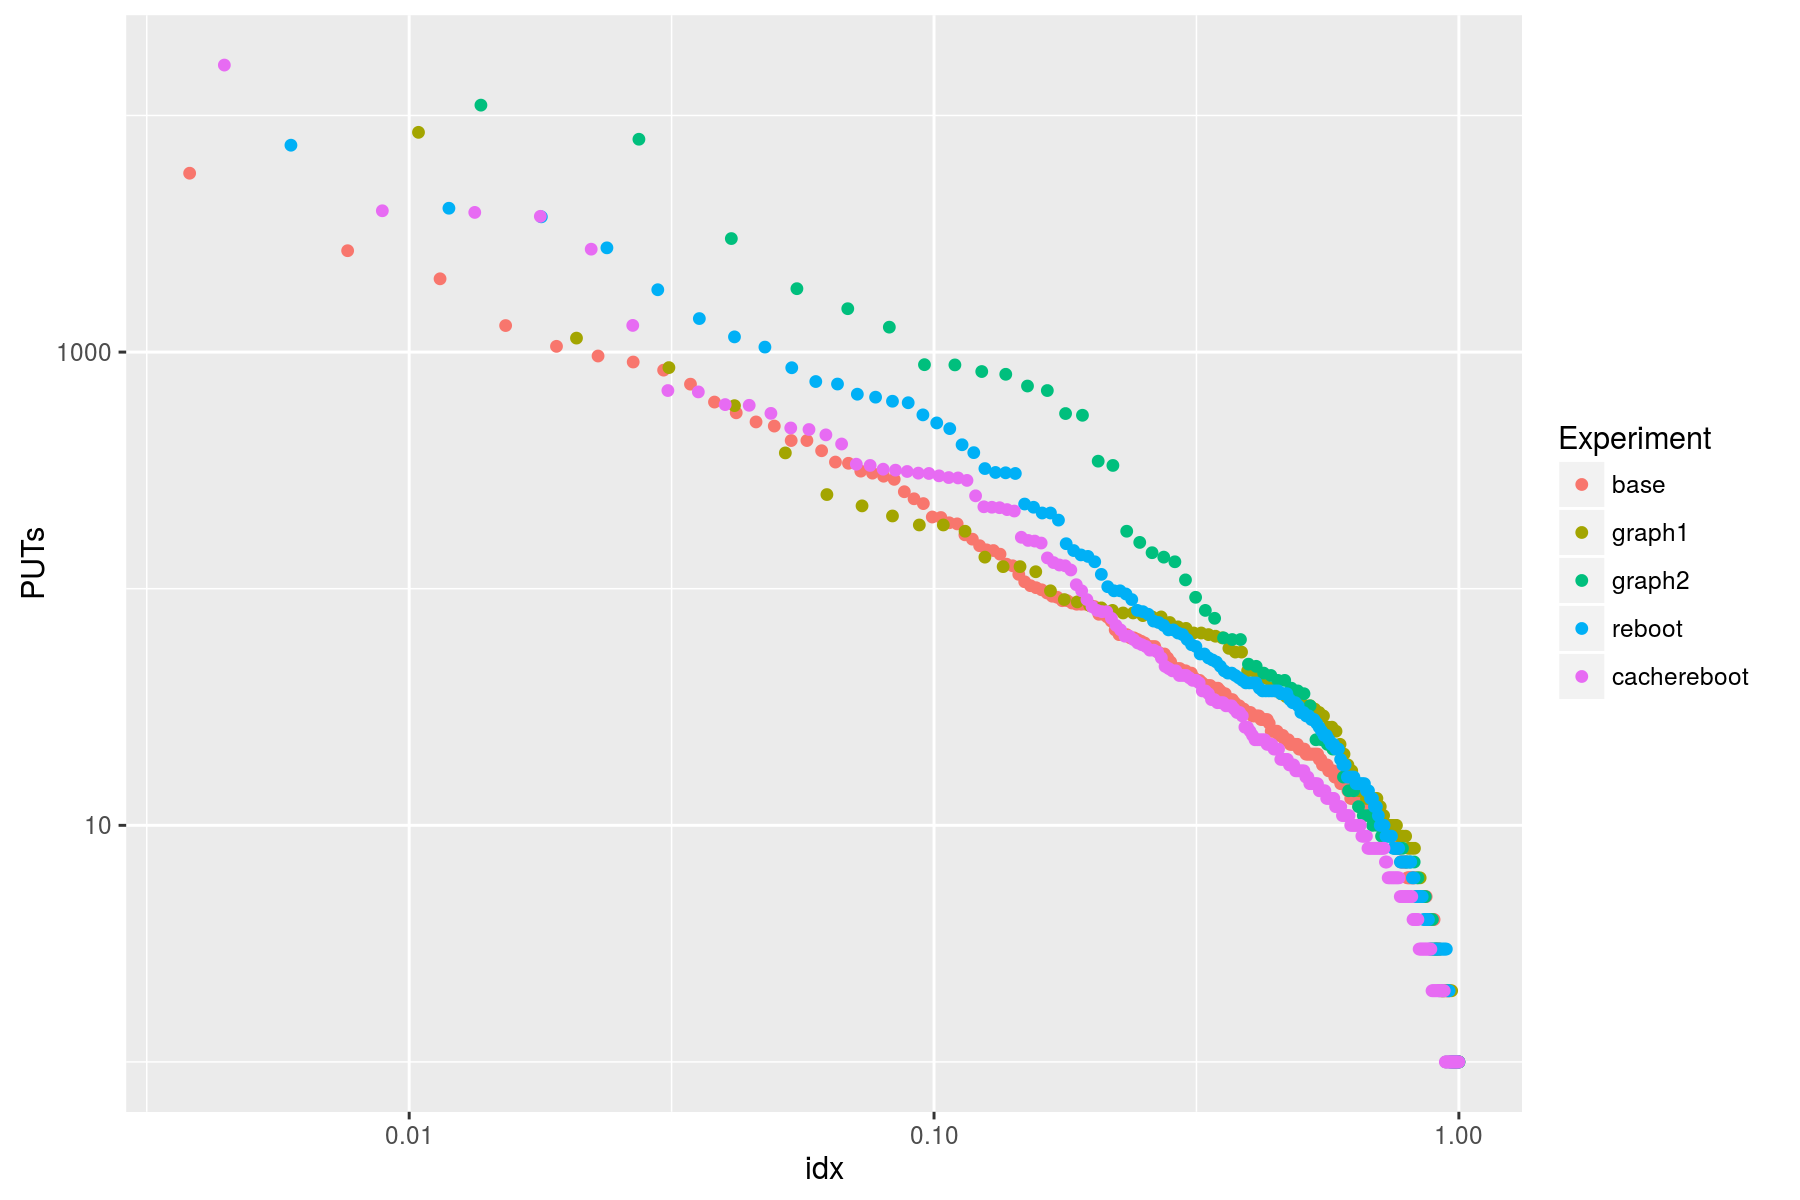
\includegraphics[width=\maxwidth]{figure/zipf-1} 

\end{knitrout}
%
\caption{Log-log plot of ranked and normalized number of contributions (PUTs) per IP.\label{fig:zipf}}
\end{figure}
%
Every run had slightly different conditions, although in some cases it
was just a server reboot and a new round of announcements. Each run
batch included at least 30 completions, that is, evolution until the
solution was found. The number of runs was controlled by polling an
URL that indicated the number of runs made in the present batch so
far. Every volunteer contributed a certain number of individuals
(represented by the PUT HTTP request) to the server. The ranked number
of contributions per unique IP is shown in Figure \ref{fig:zipf} in a
log-log scale. Besides following the usual Zipf's law found in our
previous work and thus having a very similar appearance for all 5 sets, it
is interesting to see how some sets have a number of contributions per
IP that are slightly superior to the rest, especially so in {\tt
  graph2}. The last two sets, {\tt reboot} and {\tt cachereboot}, also
show a regime in the middle of the graph that shows that some users
are contributing more than in other similar sets. In general, these
differences in behavior are due more to the specific users that show
up in these experiments than to general laws, but it should also be
noted that those behaviors can be encouraged by design.

A summary of the experiments and  their results is shown in Table
\ref{tab:runs}. This table shows the median time needed to find the
solution as well as the median number of IPs and PUTs. In this case we
distinguish between the total number of clients participating in every
particular run, and the {\em actual} number whose contributions were
accepted into the cache, which was set up to accept those only if {\em
  new} chromosomes were sent to the server in order to avoid overlaps
between one run and the next. That is why, in both cases, the
``Contributing'' column includes a value that is less than the total
number. The next column includes the total number of runs in that
particular batch, finished roughly after a minimum number of 30 was reached. 

The baseline, called {\em base} in the Table, uses the
mechanism of dropping contributions from clients if they are repeated
to avoid overlap. Clients still get a random chromosome from the
server, so they can in fact proceed with the algorithm and even finish
it. However, this was not known to the volunteer, so the fact that they were not contributing to the pool was
conveyed by inserting a graph in the client that represented the size
of the cache, labeled ``How am I contributing''. The user could
then realize there was no contribution and do something
about it. These sets of runs are labeled {\tt graph1} and 2. However, a stuck
client could still add to the pool if it found a new optimum, so we
added a mechanism for rebooting the client, that is, reloading the
page, if the cache size was found to be less than 1, which indicated a
run recently started. This batch of runs is labelled {\tt
  reboot}. This size of the cache was not really noticed by some slow clients or too fast runs, so that in the
last case, labeled {\tt cachecrash}, clients rebooted if the cache
collapsed by more than a certain length, indicating a cache that had
been voided and was filling again. Our objective was twofold: to
encourage engagement by the users and also to increase the involvement
of every client in the common experiment, eliminating at the same time
overlaps between runs. 

%
\begin{table}
  \caption{Experiments with {\em overlapped} runs filtered out: summary of results. \label{tab:filtered}}
\begin{center}
\begin{tabular}{|l|c|c|c|c|c|c|c|}
\hline
Experiment & Median Time & \multicolumn{2}{|c|}{Median IPs} &\multicolumn{2}{|c|}{Median PUTs} & \#Runs &  Puts/IP \\
&   (ms)        & Total & Used & Total & Used &  & \\
\hline
base & 293685 & 13.0 & 8.0 & 483.0 & 57.0 & 47 & 35.50000\\
\hline
graph1 & 768053 & 12.0 & 5.0 & 601.0 & 79.0 & 21 & 45.84615\\
graph2 & 1477969 & 6.0 & 4.0 & 901.0 & 52.0 & 25 & 149.42857\\
\hline
reboot & 799471 & 9.5 & 6.5 & 656.5 & 67.0 & 44 & 76.48016\\
\hline
cachereboot & 463347 & 12.0 & 12.0 & 638.5 & 80.5 & 52 & 44.25911\\
\hline
\end{tabular}
%% Initially generated with this code, 
%%<<experiments.filtered, cache=FALSE,echo=FALSE>>=
%%experiment.aggregates.filtered$Experiment <- c("base","graph1","graph2","reboot","cachereboot")
%%kable(experiment.aggregates.filtered)
%%@ %def 
%
\end{center}
\end{table}
%
The first thing we will have to check is whether we have effectively eliminated these
overlaps. In order to do that, we will have to establish a threshold
under which we can reasonably expect that the solution cannot be found. In every
evolutionary algorithm it might happen, by chance, that the solution
is found in just a few evaluations, but that is usually not the
case. By looking at the logs in the last case we have established that
minimum as 16 PUTs; in less than 1600 generations no solution to that
difficult problem will be found. Let us filter then the runs,
eliminating those that used less than 1600 generations to find the
solution which can reasonably be said that they did so because some
browser ``carried over'' a chromosome from the previous run. The
results are shown in Table \ref{tab:filtered}. The first change is in
the column \#Runs, that shows that most of the runs in the initial
configurations found the solution thanks to these carried over
clients. However, in the last two rows, the ones that rebooted clients
when they detected changes in cache, the difference is minimal. This
means that one objective has been reached: if clients reboot when they
detect changes in the cache that imply a new run, overlaps are almost
eliminated. Going back to Table \ref{tab:runs}, we can see than the
ratio of effective contributions, those that feed the cache, increases
from around 13\% in the first case to almost 16\% in the last,
reaching lows of less than 6\% in some cases ({\tt graph2}). This
indicates that rebooting the clients has the positive effect of
increasing the contribution of clients to the common pool. However, we
should remark that the clients will still stop contributing if they
get stuck in a particular solution, so the ratio keeps being low
resulting in a slow change in the cache and a lower diversity of
clients that tap that cache. At any rate, an increased number of
effective PUTs will have a positive impact on the algorithm.

\begin{table}[htbp]
  \caption{Minute-wise correlation for number of participating volunteers. \label{tab:correlation}}
\begin{center}
\begin{knitrout}
\definecolor{shadecolor}{rgb}{0.969, 0.969, 0.969}\color{fgcolor}
\begin{tabular}{l|r}
\hline
Experiment & correlation\\
\hline
base & 0.8408602\\
\hline
graph1 & 0.7346538\\
\hline
reboot & 0.7280738\\
\hline
cachereboot & 0.4657099\\
\hline
\end{tabular}


\end{knitrout}
\end{center}
\end{table}
%
We can check this impact by looking at the column that refers to
median time in Table \ref{tab:filtered} and its relation to the median
number of PUTs, which reflects the number of evaluations performed by
the clients. The last two rows have a low number of evaluations,
around 650, which is higher than the first two, probably due to the
lower volunteer supply, but better than the middle one; besides, the
amount is remarkably similar. But in the last case, it takes much less
time to find the solution {\em using the same number of
  evaluations}; the same situation applies if we compare {\tt graph1}
to {\tt cachereboot}. All variables are difficult to control in this
environment, but it might be due to the fact that parallelism has
increased, there are more volunteers contributing at the same time. In
fact, as it can be seen in the last column, the median number of
contributions per user is the lowest for {\tt cachereboot}, which
needs less contributions by users to
find the same solution. Besides, the last row shows that {\em all}
users actively contribute to the cache, while in the {\tt reboot}
strategy 30\% of users do not. This might be due to the fact that {\tt
  reboot} only does so when cache size is less than one, indicating
that this strategy is only partly successful in avoiding overlaps.  

In fact, Table \ref{tab:correlation}, which shows
the correlation between the number of IPs from one minute to the
next, presents a similar  behavior for all experiments but the last one. A high correlation indicating that the number of volunteers changes
slowly from one minute to the next; however, the {\tt cachereboot} experiment correlation indicates a bigger
dynamism, with volunteers joining and leaving the experiment all the
time, maybe because experiments take less time and need less resources.

\section{Finding the keys to a good performance}
%
%
\begin{figure}[ht!b]
\centering
\begin{knitrout}
\definecolor{shadecolor}{rgb}{0.969, 0.969, 0.969}\color{fgcolor}
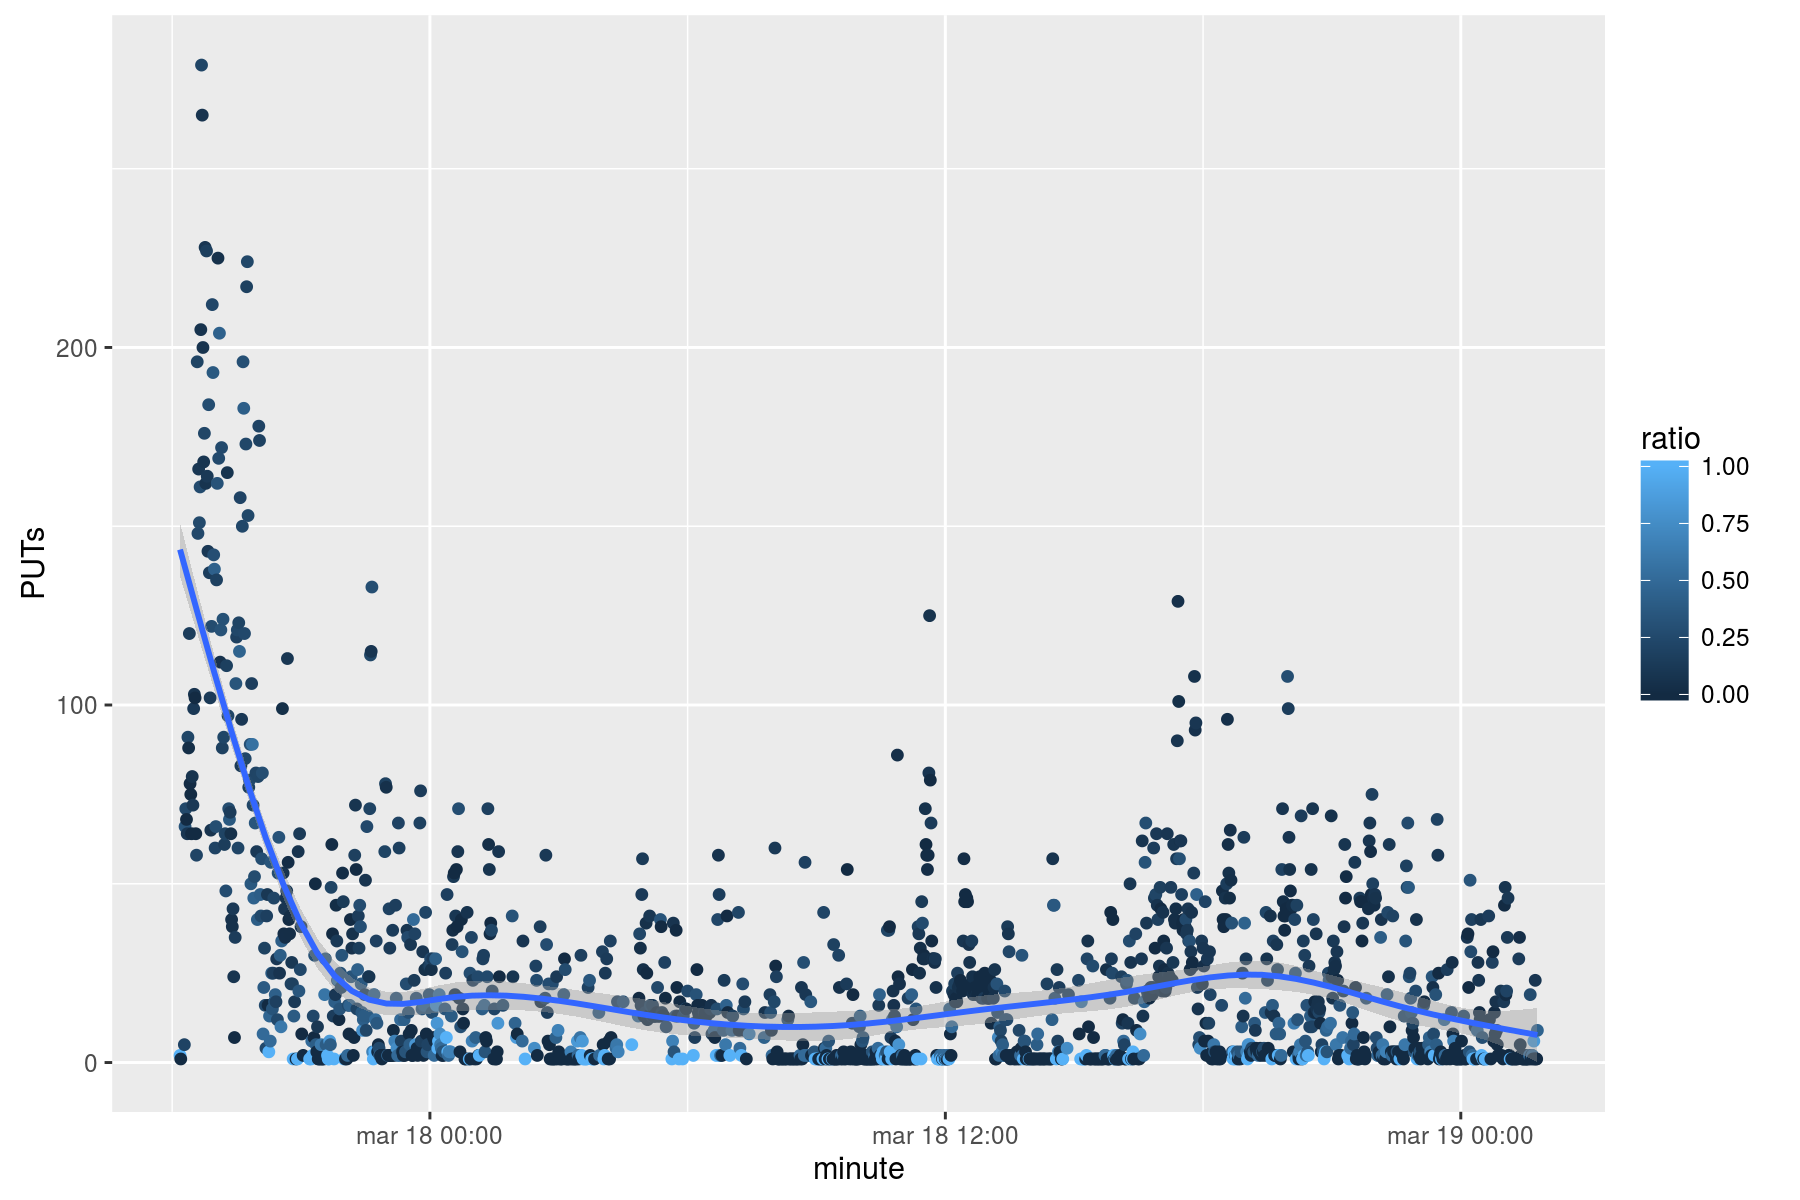
\includegraphics[width=\maxwidth]{figure/minutedata-1} 

\end{knitrout}
%
\caption{Plotting the contributions per minute in a new and massive
  experiment, as well as the real number as color. Lighter color
  indicates that all PUTs contributed new individuals to the
  experiment, darker color few to none. \label{fig:minute}}
\end{figure}

In order to have enough data to perform more analysis on it, a new
experiment was performed along several days with, eventually, several
hundreds of persons participating on it. It was announced by several
popular Twitter figures and found its way into Reddit. The number of
PUTs per minute are shown in \ref{fig:minute}. Sudden peaks in them
are due to new announcements in social networks, usually; this is one
of the problems with this kind of volunteer computing systems: they
feed on the continuous influx of new users; however, this can be
automatized and also encouraged, and, as shown, once enough users have
participated it is sometimes easier to find new ones. 

In Figure \ref{fig:minute} check
also the dot color, which 
corresponds to the {\em ratio} or, as indicated above, the actual
number of contributing PUTs, those that have not been discarded due to
repeated sending by clients or (briefly) belonging to the previous
instance of the experiment. It reveals that, in some cases where the
amount of PUTs really increases, they are actually not contributing so
much, while light dots, corresponding to a ration close to 1, usually
stay in the lowest part of the graphic. 
%
\begin{figure}[ht!b]
\centering
\begin{knitrout}
\definecolor{shadecolor}{rgb}{0.969, 0.969, 0.969}\color{fgcolor}
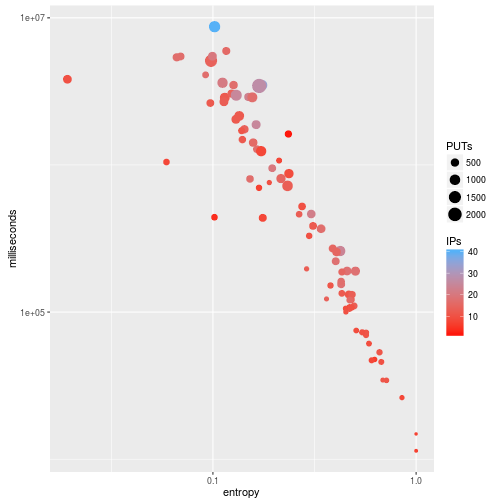
\includegraphics[width=\maxwidth]{figure/entropy-1} 

\end{knitrout}
%
\caption{Entropy of the user contribution vs. time to solution in the
  volunteer computing experiment. The fit to a linear model is significant. \label{fig:entropy}}
\end{figure}

This is interesting in the sense that in indicates that there might be
something more to performance that just the number of volunteers
contributing. In this experiment we include an additional measure:
user-contribution entropy, which is measure by computing the
compression entropy of the user contributions every for the whole
experiment.  This is computed converting the sequence of the number of
PUTs into a string and then compressing it using {\tt Zlib}, a
standard compression library. Since the compression rate is related to
the randomness of the sequence, a higher compression rate will
correspond to an experiment with a low entropy, while a lower
compression rate will indicate that there has been a certain amount of
unexpected changes during the experiment. Although less popular than
Jenssen-Shannon entropy, this way of measuring it is widely used
\cite{ornstein1993entropy} in case where we want to compute the
entropy of sequences of events, such as arrhythmias
\cite{baumert2004forecasting}. Unlike Jenssen-Shannon entropy, the
range of the compression entropy will vary between 0 (lower, or worse
compression rate) and 1 (no compression). 

The graph that plots the time to solution of every instance of the
experiment vs. entrop is shown in \ref{fig:entropy}. There is a clear
trend towards experiments with lower entropy taking more time and
experiments with higher entropy taking more time, which indeed can be
statistically fit to a linear model. This dependence on entropy is
much clearer than the assumed dependence on the number of users, which
is represented in the graph by dot color, and even the number of PUTs
or contributions, which is represented by dot size. You can see a
clearly blue and big dot, meaning more than 40 different IPs
participating and around 1500 PUTs in the high end of the graph,
showing that it took the longest to find the solution. On the other
hand, clearly red and small dots are on the lowest end of the graph,
indicating that it took a short time to find the solution as long as
the entropy is high. 

This is a very significant result which has many implications on
volunteer computing experiment design, and is clearly something that
has to do more with the fact that we are dealing with an evolutionary
algorithm where creating and maintaining diversity is an important
part of its exploration component, than with the fact that it is a
volunteer computing experiment. This is why we claim that volunteer
computing setups are, in some cases, a better option than synchronous
and distributed implementations with a similar computing capability,
because if diversity is kept high, the performance achieved can be
much better than in similar synchronous and parallel experiments. 


%---------------------------------------------------------------
\section{Conclusion}
\label{sec:conclusion}

Our main intention in this paper was to configure an evolutionary
algorithm in a volunteer computing environment to improve its
efficiency and eventually find out what this efficiency depends
on. The baseline configuration that we had used in other papers  included
{\em overlaps} or volunteers running islands that had actually started in
a previous experiment instance in the set. In previous papers, we were
interested in measuring the number of users or their behavior in bulk
and this overlap was not so important, but
in this case our focus was on the evolutionary algorithm so we had to
make all volunteers in it started more or less at the same time and
from a random population. In fact, we managed to do so, except in some
byzantine cases, by making the clients restart when the cache size
collapses to 1 or to a size much smaller than the current; we called
this client configuration {\tt reboot} and {\tt cachecrash}.  This
configuration achieves a positive secondary effect: all clients
contribute to fill the cache, having thus an actual effect on the
chromosome pool and effectively making all clients present contribute
to the simulation. 

The last configuration managed to find, with a relatively small number
of evaluations, solutions in half the time that in previous sets of
experiments. Although in the {\tt base} and {\tt graph} the median
time and number of contributions was smaller, we cannot disregard the
possibility that many of those solutions were found thanks to
contributions from {\em carried over} islands with an algorithm that
has run a big amount of evaluations already. At any rate, the {\tt
  cachereboot} finds on average solutions four times as fast as {\tt
  graph2} with twice as many average volunteers (or three times as
many if we consider {\em effective} volunteers), needing 50\% less
evaluations, thus meaning a big improvement in the performance of the
evolutionary algorithm, which was the target of this paper. This
improvement is less with respect to {\tt reboot}, but in any case the
method to detect the beginning of a new run is much more effective and
will be kept in the future. But the fact that this happened was due to
the {\em entropy} as proved in the last section of this paper. 

This future work holds many challenges which once again will go in two
different directions: gathering more users and improving the
efficiency of the algorithm run in an asynchronous way by the
users. In the first case, it will be interesting to make it more {\em
  social} by comparing local performance to other's contributions, and
showing it in a graph or being able to tweet advances or the fact that
the solution has been found. Anything that keeps the users running the
system and attracts new users will contribute to the speed of finding
the solution. And the algorithm will have to be improved, mainly by
making the population more diverse. Right now there is a rigid policy
of contribution to the pool: send the best individual, but this could
be relaxed. Some other policies could also be tested, as well as
running heterogeneous algorithms in the same way that was done in
\cite{DBLP:journals/grid/ValdezTGVO15}. Diversity, as in any other
evolutionary algorithm, seems to be the key, but there are many ways of
approaching it. 

All these avenues of experimentation will be done openly following the
Open Science policy of our group, which, in fact, contributes to
establish trust and security between us and volunteers and is an
essential feature of the system. That is why this paper, as well as
the data and processing scripts, are published with a free license in GitHub at
\url{ANONYMOUS-URL}.
%\url{https://git.io/gecco-es-15}.

%---------------------------------------------------------------
\section*{Acknowledgments}

% This work has been supported in part by TIN2014-56494-C4-3-P (Spanish
% Ministry of Economy and Competitivity), PROY-PP2015-06 (Plan Propio
% 2015 UGR). We are also grateful to {\tt @otisdriftwood} for his help
% gathering users for the new experiments.

Several projects\\
Taking\\
This\\
Much\\
Space\\ 

\bibliographystyle{splncs}
\bibliography{volunteer,GA-general,geneura,javascript,ror-js}

\end{document}

%%% Local Variables:
%%% ispell-local-dictionary: "english"
%%% End:
